\documentclass[aspectratio=169,12pt]{beamer}
\usepackage[utf8]{inputenc}
\usepackage[T1]{fontenc}
\usepackage[polish]{babel}
\usepackage{carlito}
\usepackage{booktabs}
\usepackage{multirow}
\usepackage{graphicx}
\usepackage{array}
\usepackage{colortbl}
\usepackage{tikz}

\usetheme[lang=pl]{NewPwr}

% Stopka z autorami i numeracją slajdów
\setbeamertemplate{footline}{%
    \leavevmode%
    \hbox{%
        \begin{beamercolorbox}[wd=.15\paperwidth,ht=2.5ex,dp=1ex,left,leftskip=1em]{author in head/foot}%
        \end{beamercolorbox}%
        \begin{beamercolorbox}[wd=.7\paperwidth,ht=2.5ex,dp=1ex,center]{author in head/foot}%
            \usebeamerfont{author in head/foot}\insertshortauthor
        \end{beamercolorbox}%
        \begin{beamercolorbox}[wd=.15\paperwidth,ht=2.5ex,dp=1ex,right,rightskip=1em]{date in head/foot}%
            \usebeamerfont{date in head/foot}\insertframenumber{} / \inserttotalframenumber
        \end{beamercolorbox}%
    }%
    \vskip0pt%
}

\title{Przewidywanie Długości Pobytu w Szpitalu\\za pomocą Sieci Neuronowych}
\subtitle{Projekt z Sieci Neuronowych}
\author{Kamil Selega (288780), Maria Słomiany (268576), Katarzyna Szczepaniak (261895)}
\institute{Wydział Informatyki i Telekomunikacji, Politechnika Wrocławska}
\date{Styczeń 2026}

\begin{document}

%=============================================================================
\begin{frame}[plain]
    \titlepage
\end{frame}

%=============================================================================
\begin{frame}{Cel projektu}
    \begin{columns}[T]
        \begin{column}{0.5\textwidth}
            \textbf{Zadanie:}
            \begin{itemize}
                \item Przewidywanie długości pobytu pacjenta w szpitalu
                \item Problem regresji
                \item Porównanie 3 architektur sieci neuronowych
            \end{itemize}
            \vspace{0.5cm}
            \textbf{Metryki:}
            \begin{itemize}
                \item MAE (Mean Absolute Error)
                \item RMSE (Root Mean Squared Error)
                \item R² (współczynnik determinacji)
            \end{itemize}
        \end{column}
        \begin{column}{0.5\textwidth}
            \textbf{Architektury:}
            \begin{enumerate}
                \item SimpleMLP (baseline)
                \item TabNet (attention)
                \item TabTransformer (self-attention)
            \end{enumerate}
            \vspace{0.5cm}
            \textbf{Metodologia:}
            \begin{itemize}
                \item Grid Search
                \item 5-fold Cross-Validation
                \item 62 konfiguracje łącznie
            \end{itemize}
        \end{column}
    \end{columns}
\end{frame}

%=============================================================================
\begin{frame}{Dane -- Healthcare Risk Factors Dataset}
    \begin{columns}[T]
        \begin{column}{0.5\textwidth}
            \textbf{Cechy wejściowe (22):}
            \begin{itemize}
                \item Dane demograficzne (wiek, płeć)
                \item BMI, ciśnienie krwi, cholesterol
                \item Palenie, aktywność fizyczna
                \item Stan medyczny (one-hot encoding)
            \end{itemize}
            \vspace{0.3cm}
            \textbf{Zmienna docelowa:}
            \begin{itemize}
                \item Długość pobytu w szpitalu [dni]
            \end{itemize}
        \end{column}
        \begin{column}{0.5\textwidth}
            \textbf{Preprocessing:}
            \begin{itemize}
                \item Usunięcie kolumn szumu
                \item Usunięcie brakujących wartości
                \item Kodowanie kategoryczne
            \end{itemize}
            \vspace{0.3cm}
            \textbf{Podział danych:}
            \begin{center}
                \begin{tikzpicture}[scale=0.7]
                    \fill[blue!50] (0,0) rectangle (5.6,1);
                    \fill[red!50] (5.6,0) rectangle (8,1);
                    \node[font=\small, black] at (2.8,0.5) {\textbf{Trening: 80\%}};
                    \node[font=\small, black] at (6.8,0.5) {\textbf{Test: 20\%}};
                \end{tikzpicture}
            \end{center}
        \end{column}
    \end{columns}
\end{frame}

%=============================================================================
\begin{frame}{Architektury sieci neuronowych}
    \begin{columns}[T]
        \begin{column}{0.33\textwidth}
            \centering
            \textbf{\large SimpleMLP}
            \vspace{0.4cm}

            \begin{tikzpicture}[scale=0.85]
                \foreach \y in {0,0.5,1,1.5,2} \fill[blue!60] (0,\y) circle (0.2);
                \foreach \y in {0.25,0.75,1.25,1.75} \fill[green!60] (1.5,\y) circle (0.2);
                \fill[red!60] (3,1) circle (0.2);

                \foreach \x in {0,0.5,1,1.5,2} {
                        \foreach \y in {0.25,0.75,1.25,1.75} {
                                \draw[gray!50, thin] (0.2,\x) -- (1.3,\y);
                            }
                    }
                \foreach \y in {0.25,0.75,1.25,1.75} {
                        \draw[gray!50, thin] (1.7,\y) -- (2.8,1);
                    }
            \end{tikzpicture}

            \vspace{0.3cm}
            \small
            \begin{itemize}
                \item Fully-connected
                \item Dropout
                \item ReLU/Tanh
            \end{itemize}
        \end{column}
        \begin{column}{0.33\textwidth}
            \centering
            \textbf{\large TabNet}
            \vspace{0.4cm}

            \begin{tikzpicture}[scale=0.85]
                \fill[blue!60] (0,0) rectangle (3,0.55);
                \fill[orange!60] (0,0.75) rectangle (3,1.3);
                \fill[green!60] (0,1.5) rectangle (3,2.05);
                \fill[red!60] (0,2.25) rectangle (3,2.8);

                \node[font=\footnotesize] at (1.5,0.275) {Input};
                \node[font=\footnotesize] at (1.5,1.025) {Attention};
                \node[font=\footnotesize] at (1.5,1.775) {Feature Trans.};
                \node[font=\footnotesize] at (1.5,2.525) {Output};
            \end{tikzpicture}

            \vspace{0.3cm}
            \small
            \begin{itemize}
                \item Sequential attention
                \item Feature selection
                \item Interpretowalność
            \end{itemize}
        \end{column}
        \begin{column}{0.33\textwidth}
            \centering
            \textbf{\large TabTransformer}
            \vspace{0.4cm}

            \begin{tikzpicture}[scale=0.85]
                \fill[blue!60] (0,0) rectangle (3,0.55);
                \fill[purple!60] (0,0.75) rectangle (3,1.3);
                \fill[purple!60] (0,1.5) rectangle (3,2.05);
                \fill[red!60] (0,2.25) rectangle (3,2.8);

                \node[font=\footnotesize] at (1.5,0.275) {Embeddings};
                \node[font=\footnotesize] at (1.5,1.025) {Self-Attention};
                \node[font=\footnotesize] at (1.5,1.775) {Self-Attention};
                \node[font=\footnotesize] at (1.5,2.525) {MLP Head};
            \end{tikzpicture}

            \vspace{0.3cm}
            \small
            \begin{itemize}
                \item Transformer encoder
                \item Multi-head attention
                \item Zależności między cechami
            \end{itemize}
        \end{column}
    \end{columns}
\end{frame}

%=============================================================================
\begin{frame}{Grid Search -- przestrzeń hiperparametrów}
    \begin{columns}[T]
        \begin{column}{0.33\textwidth}
            \centering
            \textbf{SimpleMLP}
            \vspace{0.2cm}

            \scriptsize
            \begin{tabular}{lc}
                \toprule
                Parametr   & Wartości        \\
                \midrule
                hidden     & [64, 128, 256]  \\
                activation & [relu, tanh]    \\
                dropout    & [0.2, 0.3, 0.4] \\
                \bottomrule
            \end{tabular}

            \vspace{0.3cm}
            \textbf{18 konfiguracji}
        \end{column}
        \begin{column}{0.33\textwidth}
            \centering
            \textbf{TabNet}
            \vspace{0.2cm}

            \scriptsize
            \begin{tabular}{lc}
                \toprule
                Parametr & Wartości    \\
                \midrule
                n\_d     & [8, 32, 64] \\
                n\_a     & [8, 32, 64] \\
                n\_steps & [3, 5, 7]   \\
                \bottomrule
            \end{tabular}

            \vspace{0.3cm}
            \textbf{27 konfiguracji}
        \end{column}
        \begin{column}{0.33\textwidth}
            \centering
            \textbf{TabTransformer}
            \vspace{0.2cm}

            \scriptsize
            \begin{tabular}{lc}
                \toprule
                Parametr    & Wartości       \\
                \midrule
                d\_model    & [64, 128, 256] \\
                n\_heads    & [2, 4, 8]      \\
                num\_layers & [1, 2, 3]      \\
                \bottomrule
            \end{tabular}

            \vspace{0.3cm}
            \textbf{17 konfiguracji}
        \end{column}
    \end{columns}

    \vspace{0.5cm}
    \begin{center}
        \textbf{Łącznie: 62 konfiguracje} $\times$ \textbf{5-fold CV} = \textbf{310 modeli}
    \end{center}
\end{frame}

%=============================================================================
\begin{frame}{}
    \begin{center}
        \vspace{1.5cm}
        {\Huge\textbf{Wyniki}}

        \vspace{1cm}
        {\large Porównanie 3 architektur sieci neuronowych}

        \vspace{0.5cm}
        {\large dla przewidywania długości pobytu w szpitalu}

        \vspace{1cm}
        \begin{tabular}{ccc}
            \textbf{SimpleMLP} & \textbf{TabNet} & \textbf{TabTransformer} \\
            (baseline)         & (attention)     & (transformer)           \\
        \end{tabular}
    \end{center}
\end{frame}

%=============================================================================
\begin{frame}{Porównanie architektur -- MAE}
    \begin{center}
        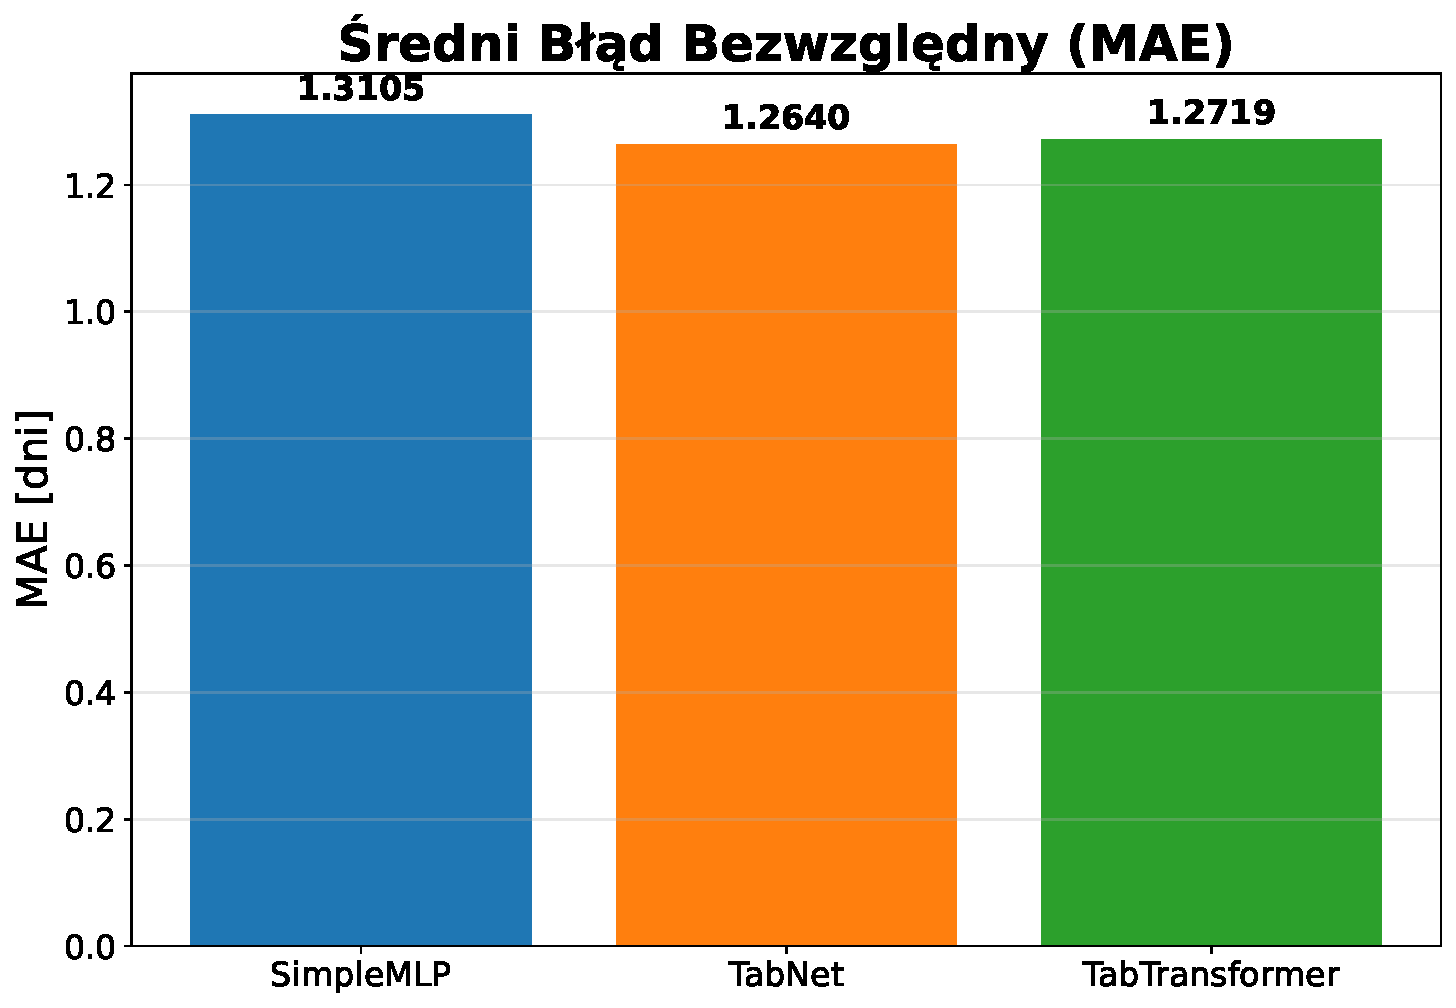
\includegraphics[width=\textwidth, height=0.82\textheight, keepaspectratio]{figures/comparison_mae.pdf}
    \end{center}
\end{frame}

%=============================================================================
\begin{frame}{Porównanie architektur -- RMSE}
    \begin{center}
        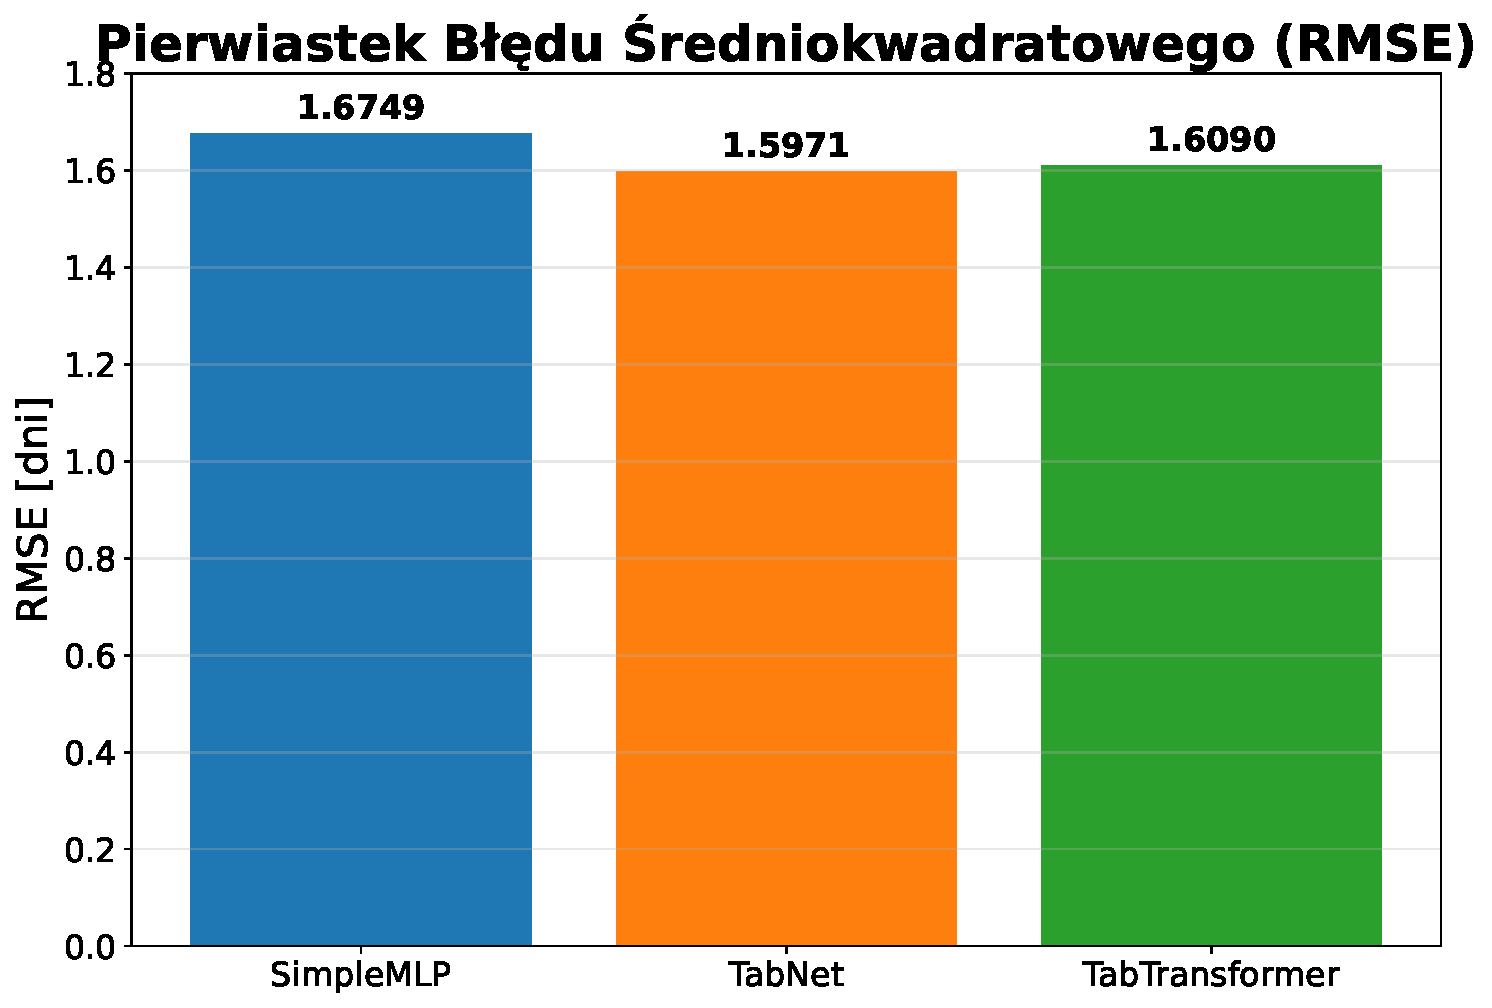
\includegraphics[width=\textwidth, height=0.82\textheight, keepaspectratio]{figures/comparison_rmse.pdf}
    \end{center}
\end{frame}

%=============================================================================
\begin{frame}{Porównanie architektur -- R²}
    \begin{center}
        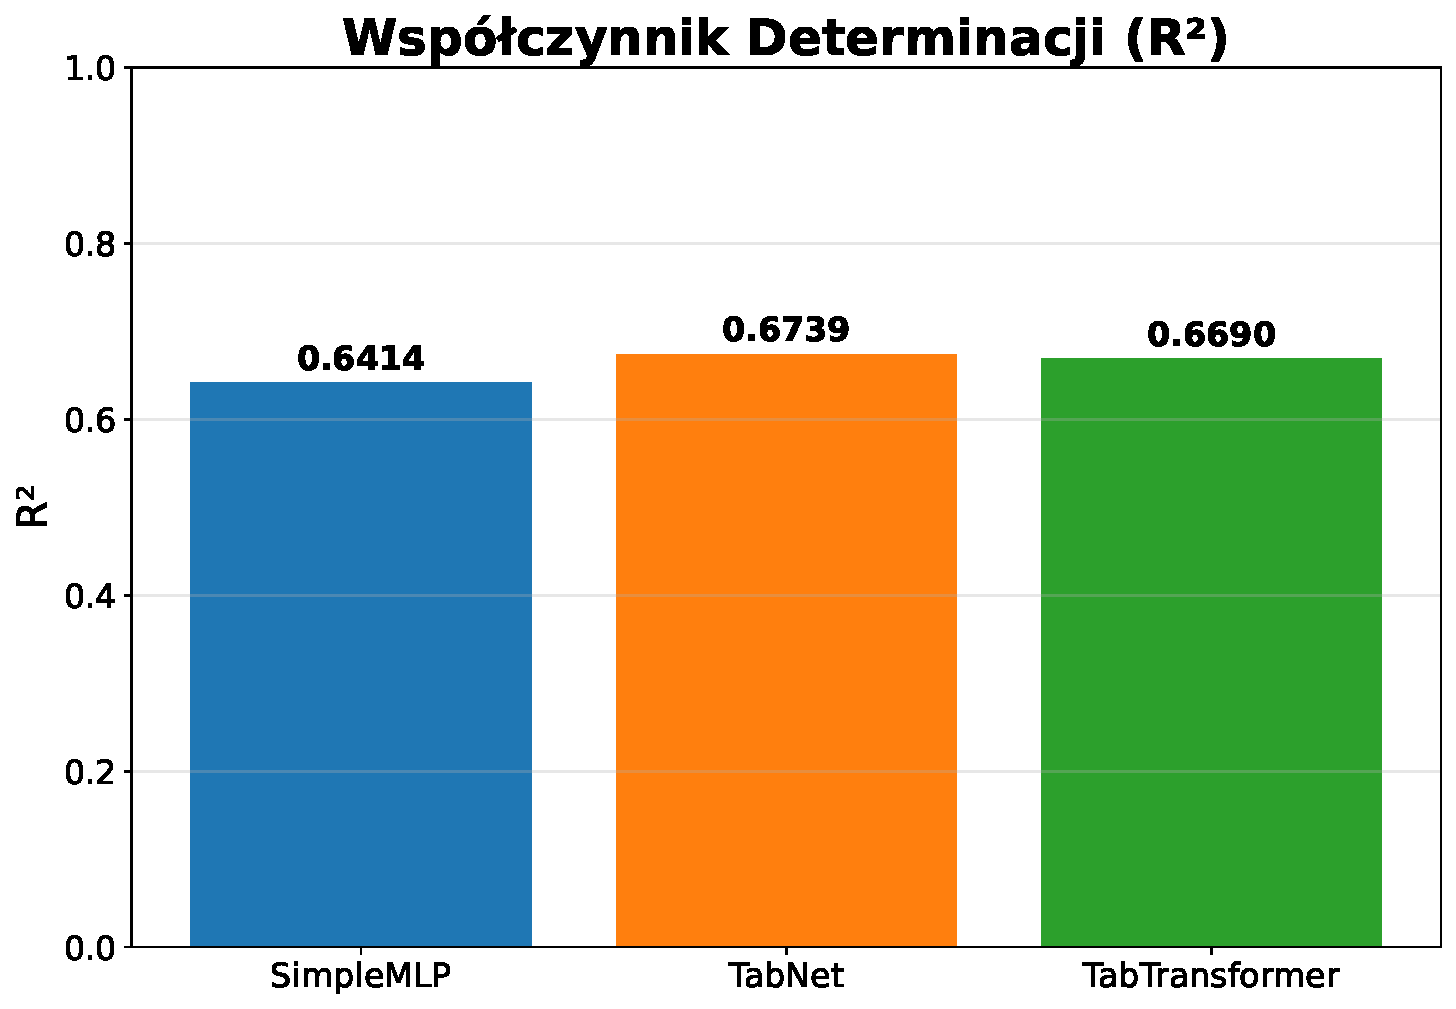
\includegraphics[width=\textwidth, height=0.82\textheight, keepaspectratio]{figures/comparison_r2.pdf}
    \end{center}
\end{frame}

%=============================================================================
\begin{frame}{Stabilność modeli w walidacji krzyżowej}
    \begin{center}
        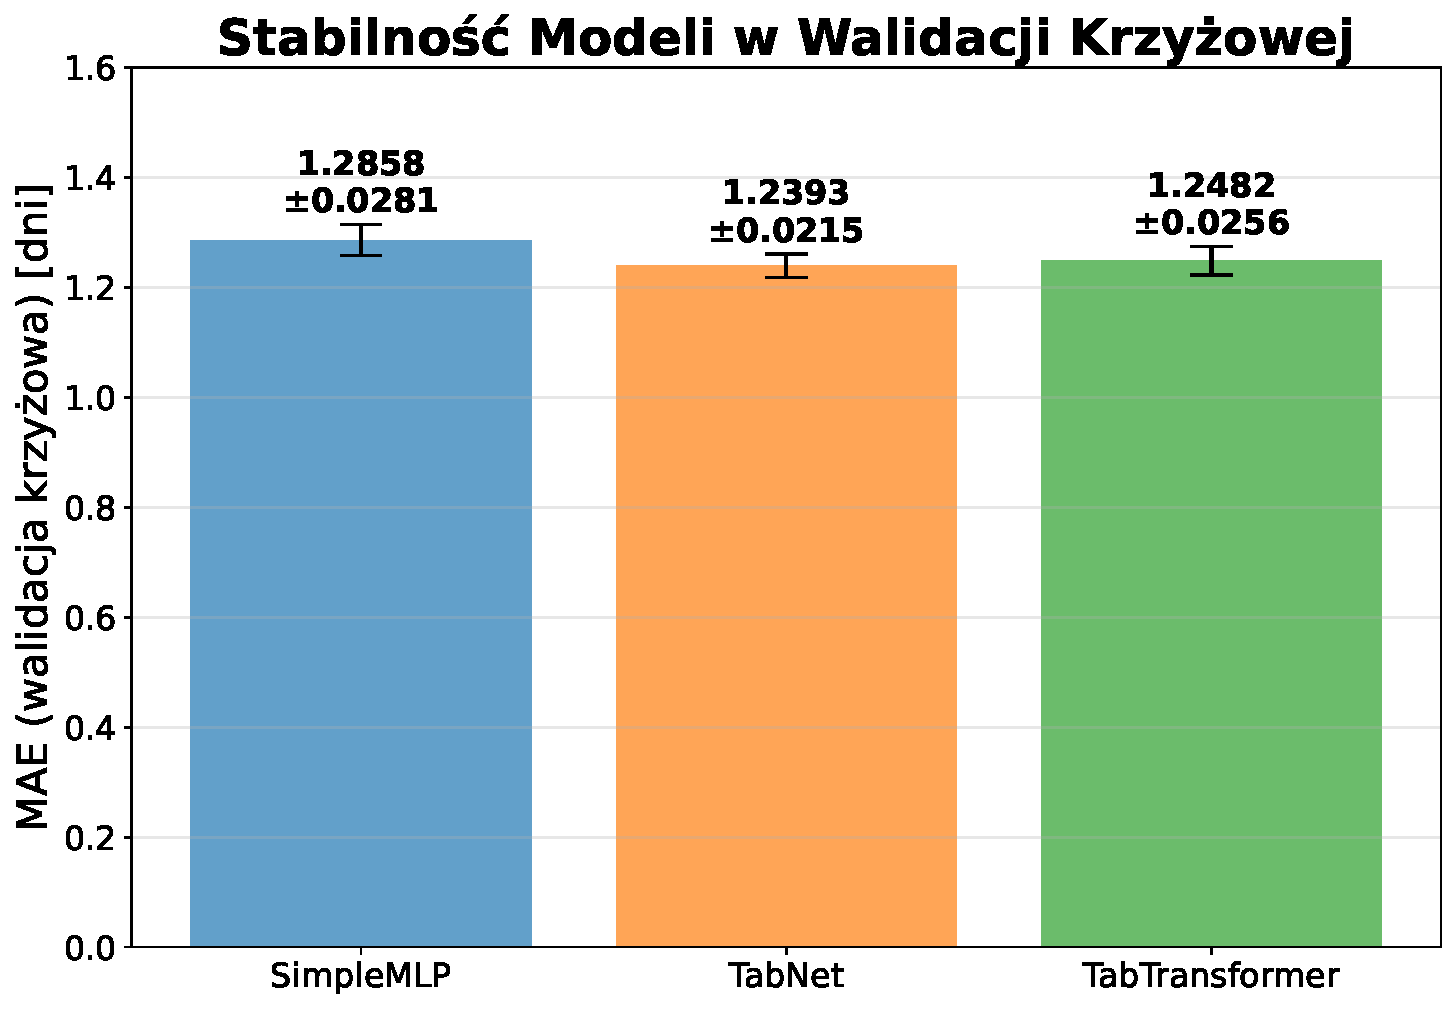
\includegraphics[width=\textwidth, height=0.82\textheight, keepaspectratio]{figures/cv_stability.pdf}
    \end{center}
\end{frame}

%=============================================================================
\begin{frame}{Wyniki -- najlepsze modele}
    \begin{center}
        \small
        \begin{tabular}{l|ccc|c}
            \toprule
            \textbf{Metryka} & \textbf{SimpleMLP} & \textbf{TabNet}                                & \textbf{TabTransformer} \\
            \midrule
            MAE (CV)         & 1.286 $\pm$ 0.028  & \cellcolor{green!20}\textbf{1.239 $\pm$ 0.022} & 1.248 $\pm$ 0.026       \\
            MAE (Test)       & 1.311              & \cellcolor{green!20}\textbf{1.264}             & 1.272                   \\
            RMSE (Test)      & 1.675              & \cellcolor{green!20}\textbf{1.597}             & 1.618                   \\
            R² (Test)        & 0.641              & \cellcolor{green!20}\textbf{0.674}             & 0.669                   \\
            \bottomrule
        \end{tabular}

        \vspace{0.5cm}
        \begin{tabular}{lc}
            \toprule
            \textbf{Najlepsze hiperparametry TabNet} & \textbf{Wartość} \\
            \midrule
            n\_d (wymiar feature transformers)       & 64               \\
            n\_a (wymiar attention layers)           & 32               \\
            n\_steps (kroki decyzyjne)               & 3                \\
            \bottomrule
        \end{tabular}
    \end{center}
\end{frame}

%=============================================================================
\begin{frame}{SimpleMLP -- Predykcje vs Wartości Rzeczywiste}
    \begin{center}
        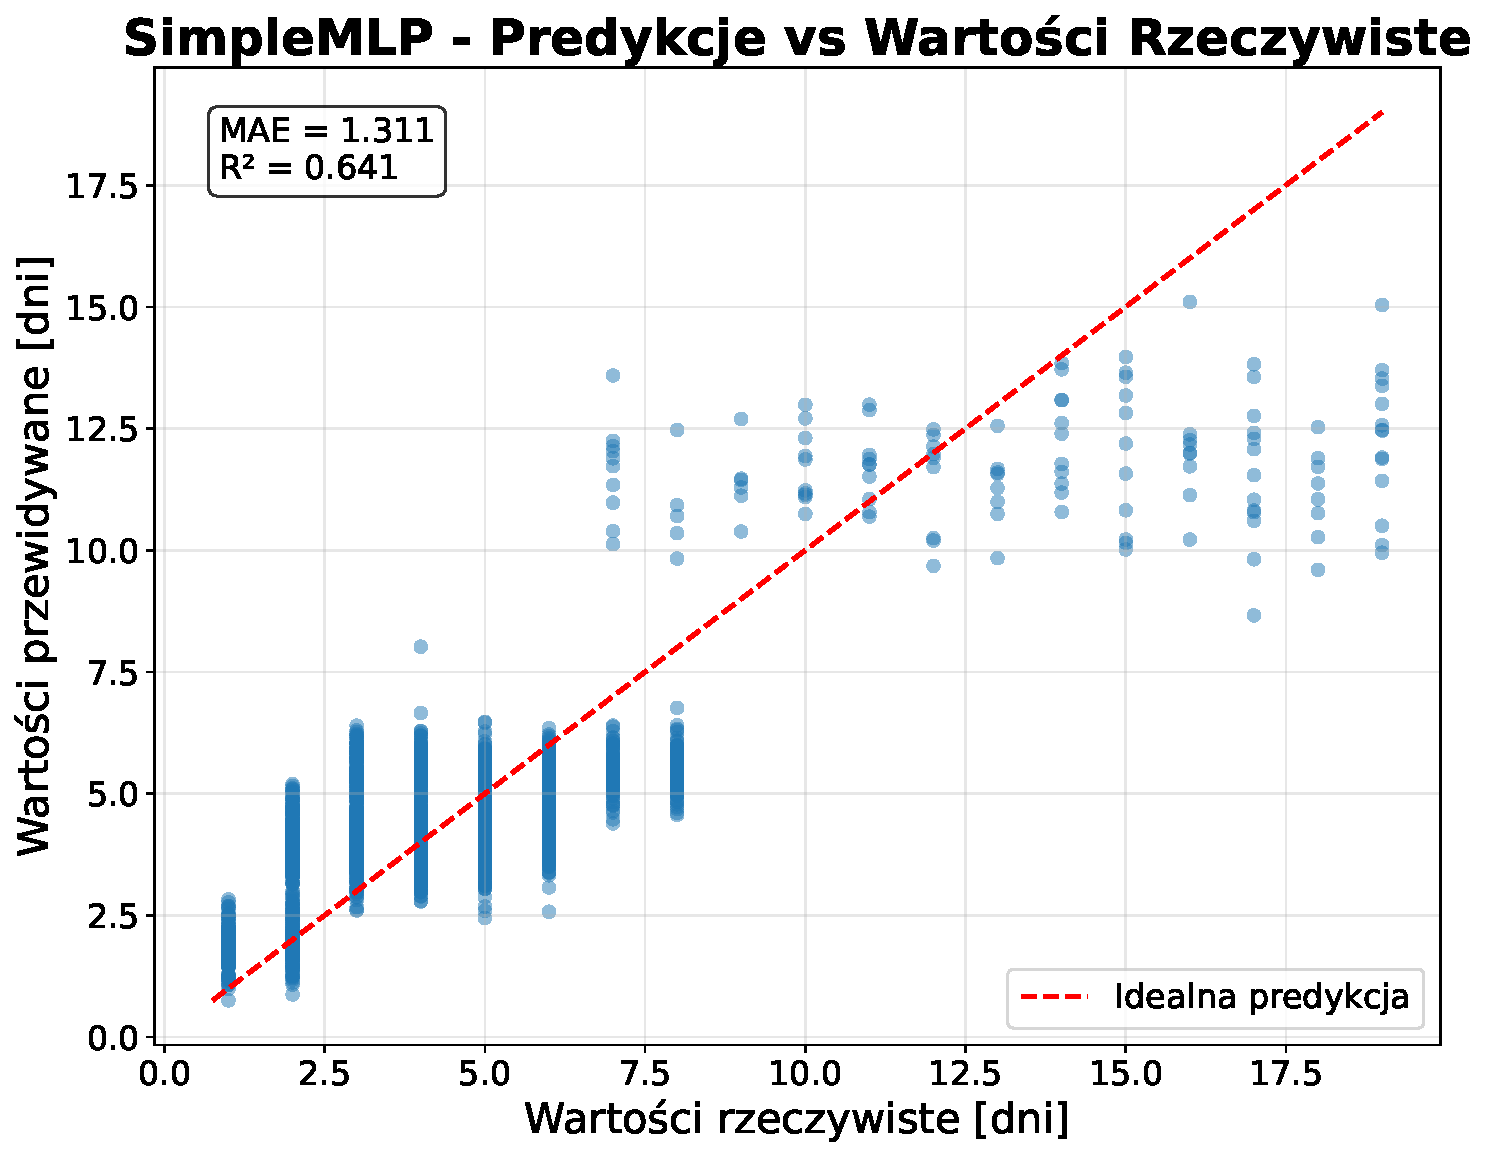
\includegraphics[width=\textwidth, height=0.82\textheight, keepaspectratio]{figures/simplemlp_predictions.pdf}
    \end{center}
\end{frame}

%=============================================================================
\begin{frame}{SimpleMLP -- Wykres Reszt}
    \begin{center}
        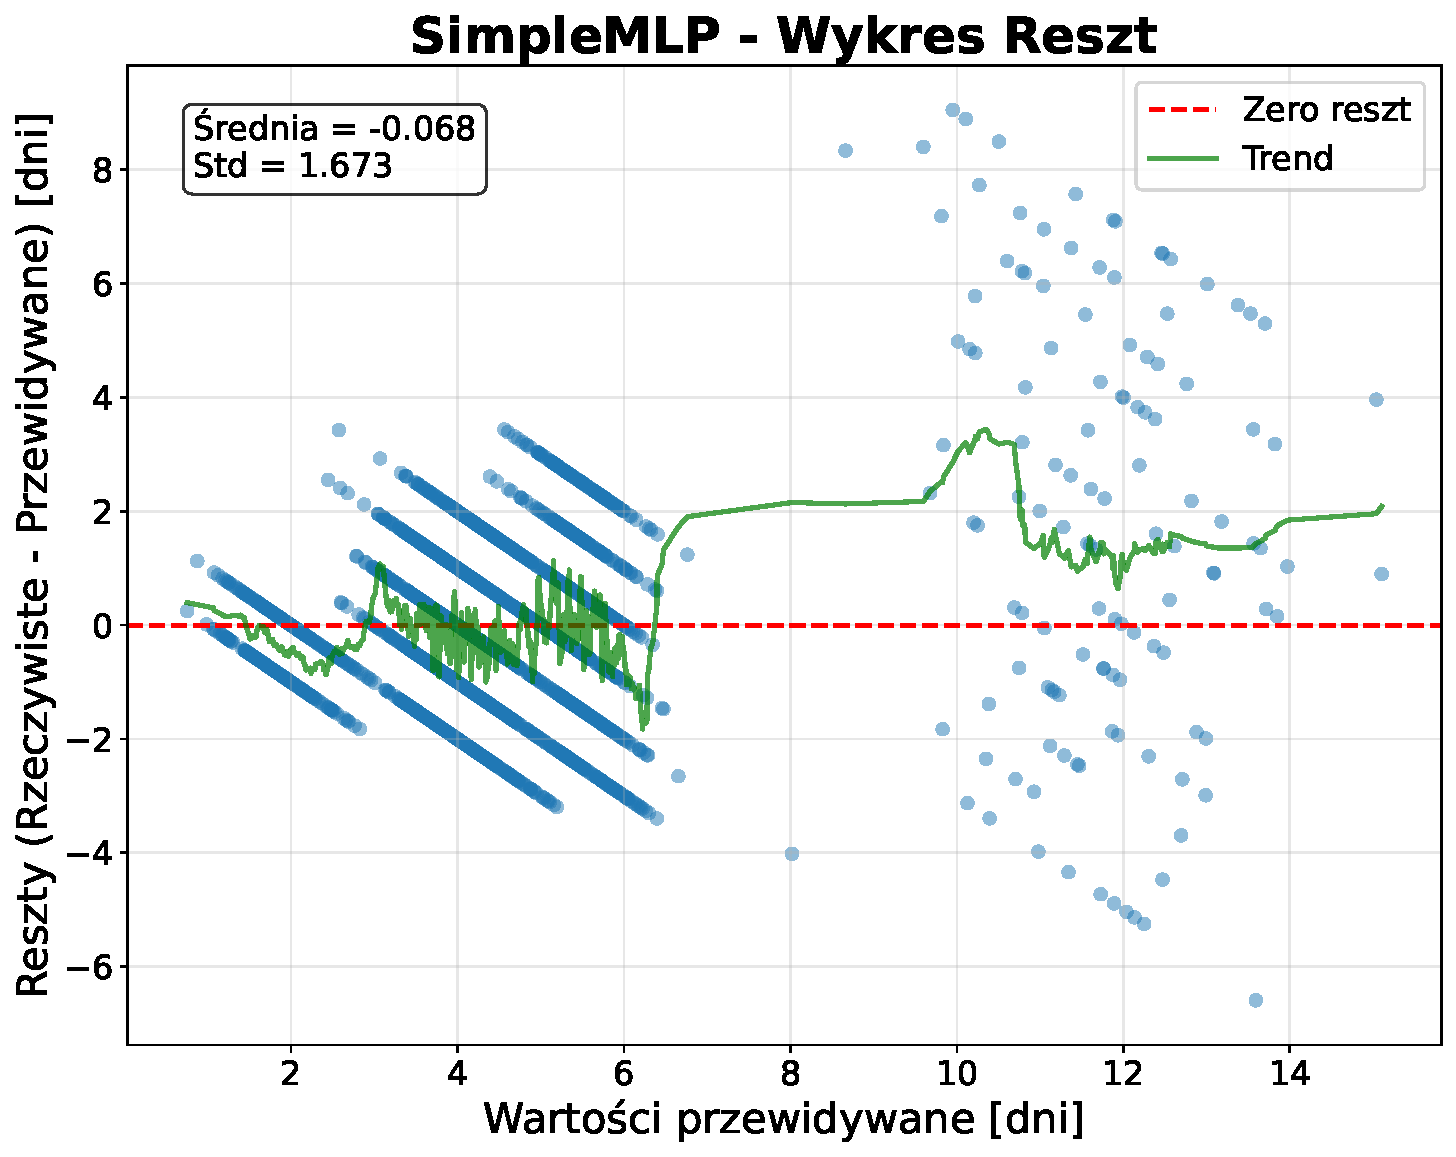
\includegraphics[width=\textwidth, height=0.82\textheight, keepaspectratio]{figures/simplemlp_residuals.pdf}
    \end{center}
\end{frame}

%=============================================================================
\begin{frame}{TabNet -- Predykcje vs Wartości Rzeczywiste}
    \begin{center}
        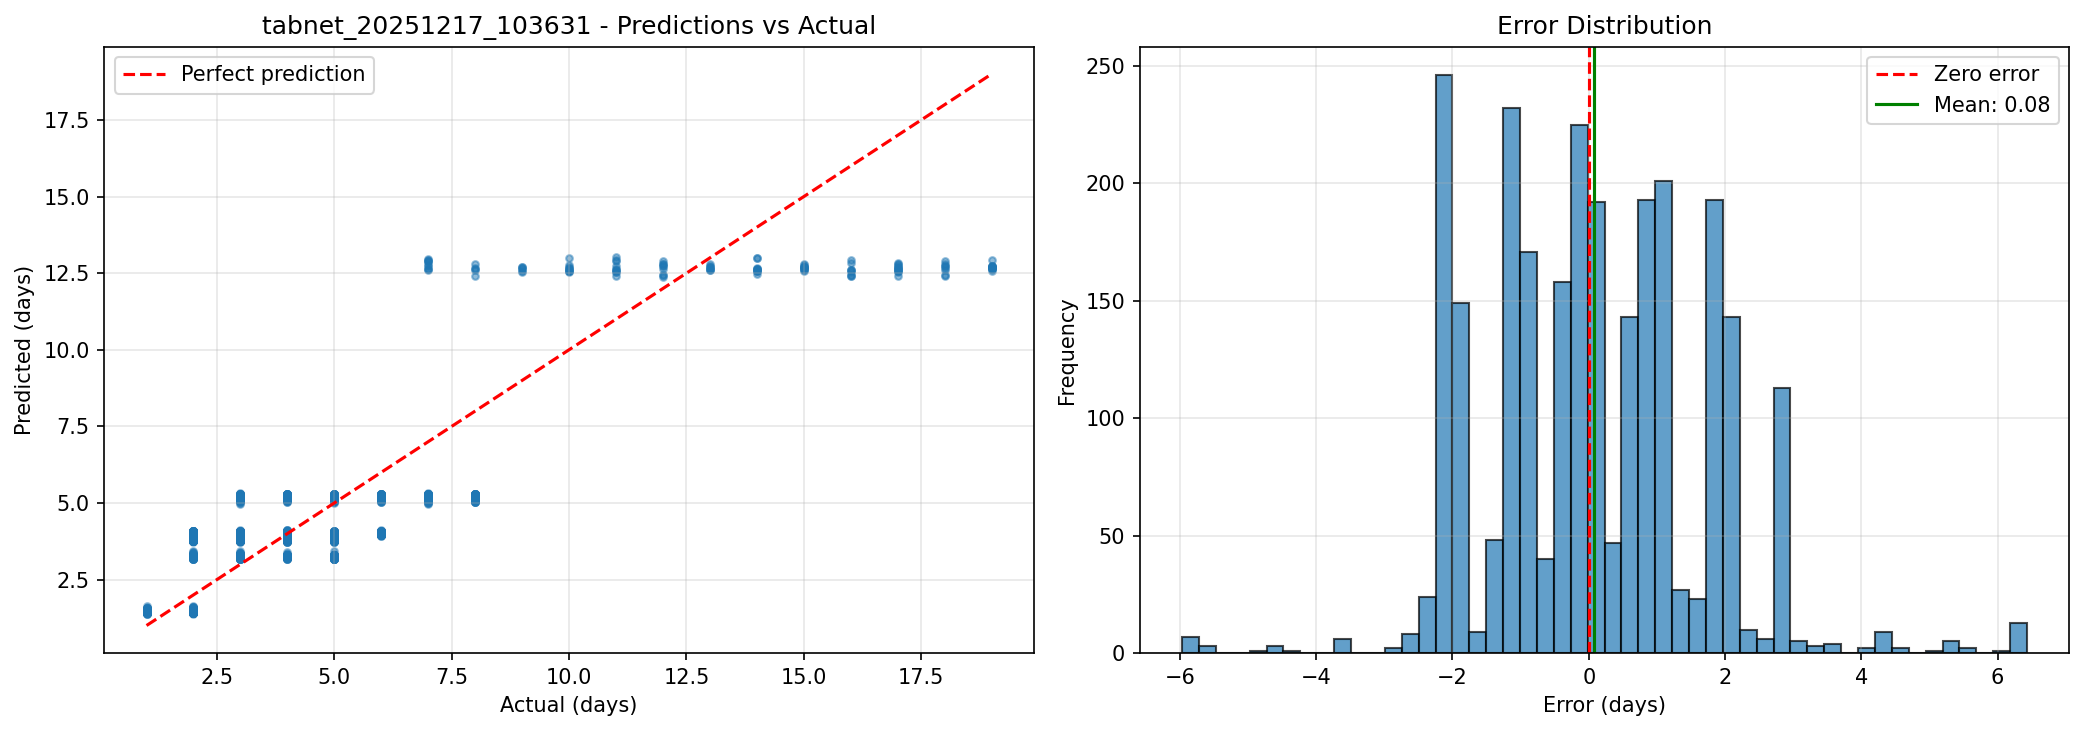
\includegraphics[width=\textwidth, height=0.82\textheight, keepaspectratio]{figures/tabnet_predictions.pdf}
    \end{center}
\end{frame}

%=============================================================================
\begin{frame}{TabNet -- Wykres Reszt}
    \begin{center}
        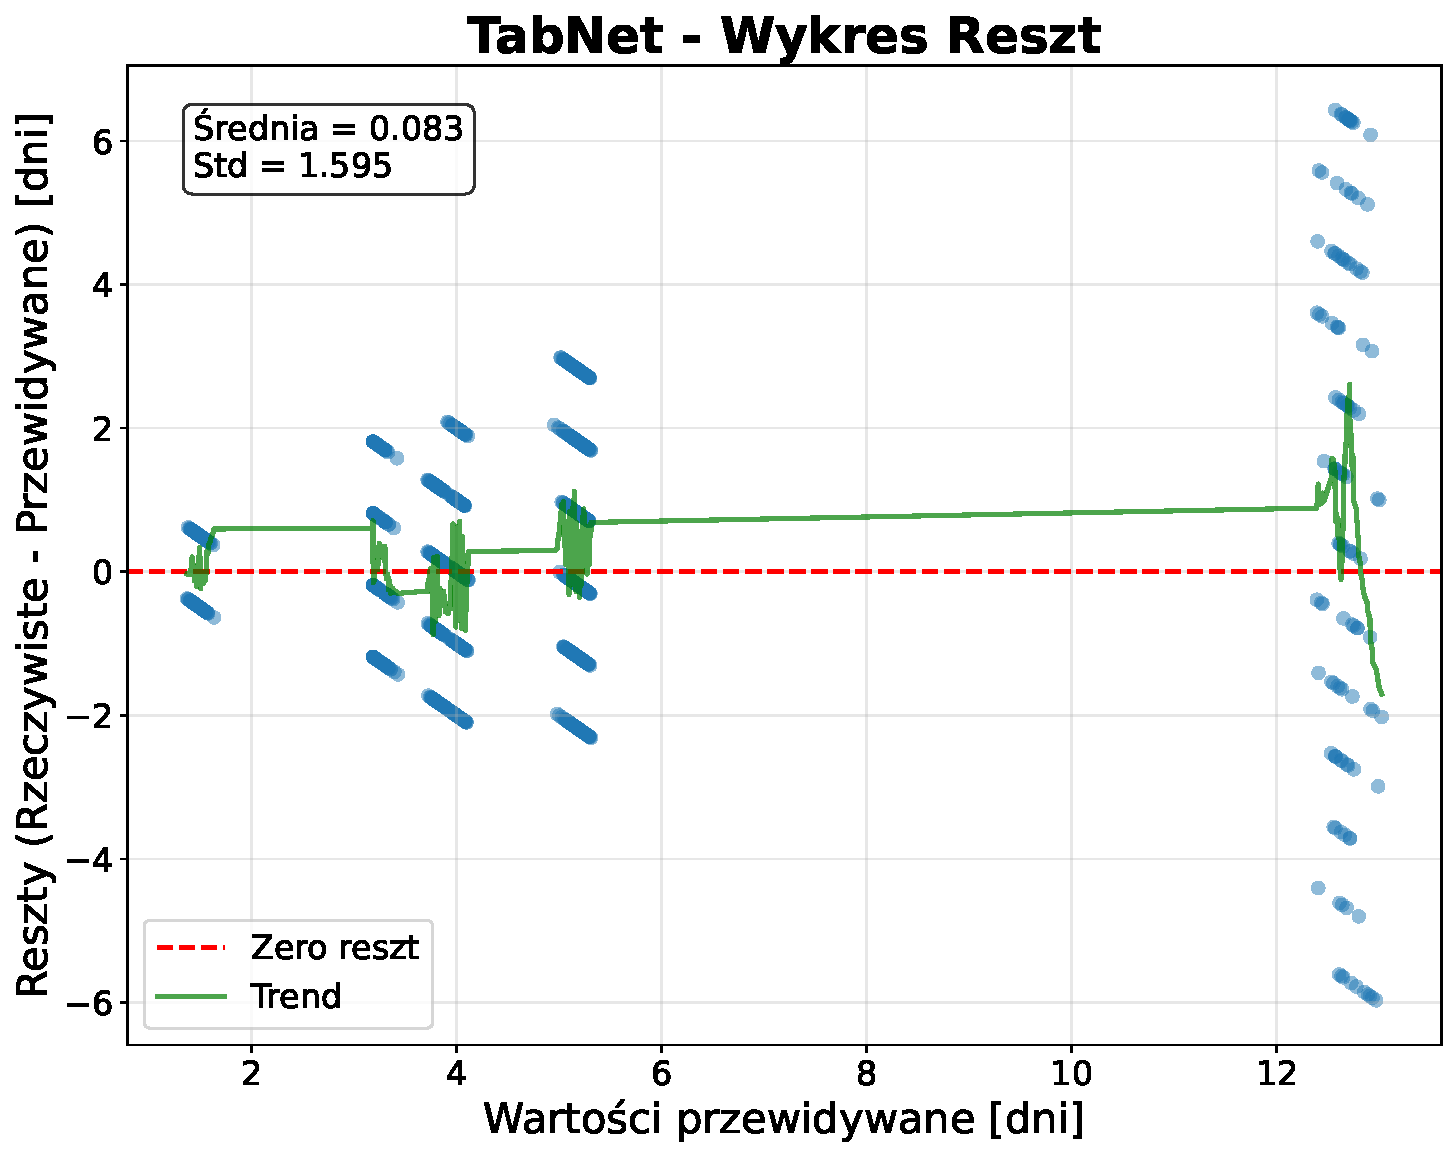
\includegraphics[width=\textwidth, height=0.82\textheight, keepaspectratio]{figures/tabnet_residuals.pdf}
    \end{center}
\end{frame}

%=============================================================================
\begin{frame}{TabTransformer -- Predykcje vs Wartości Rzeczywiste}
    \begin{center}
        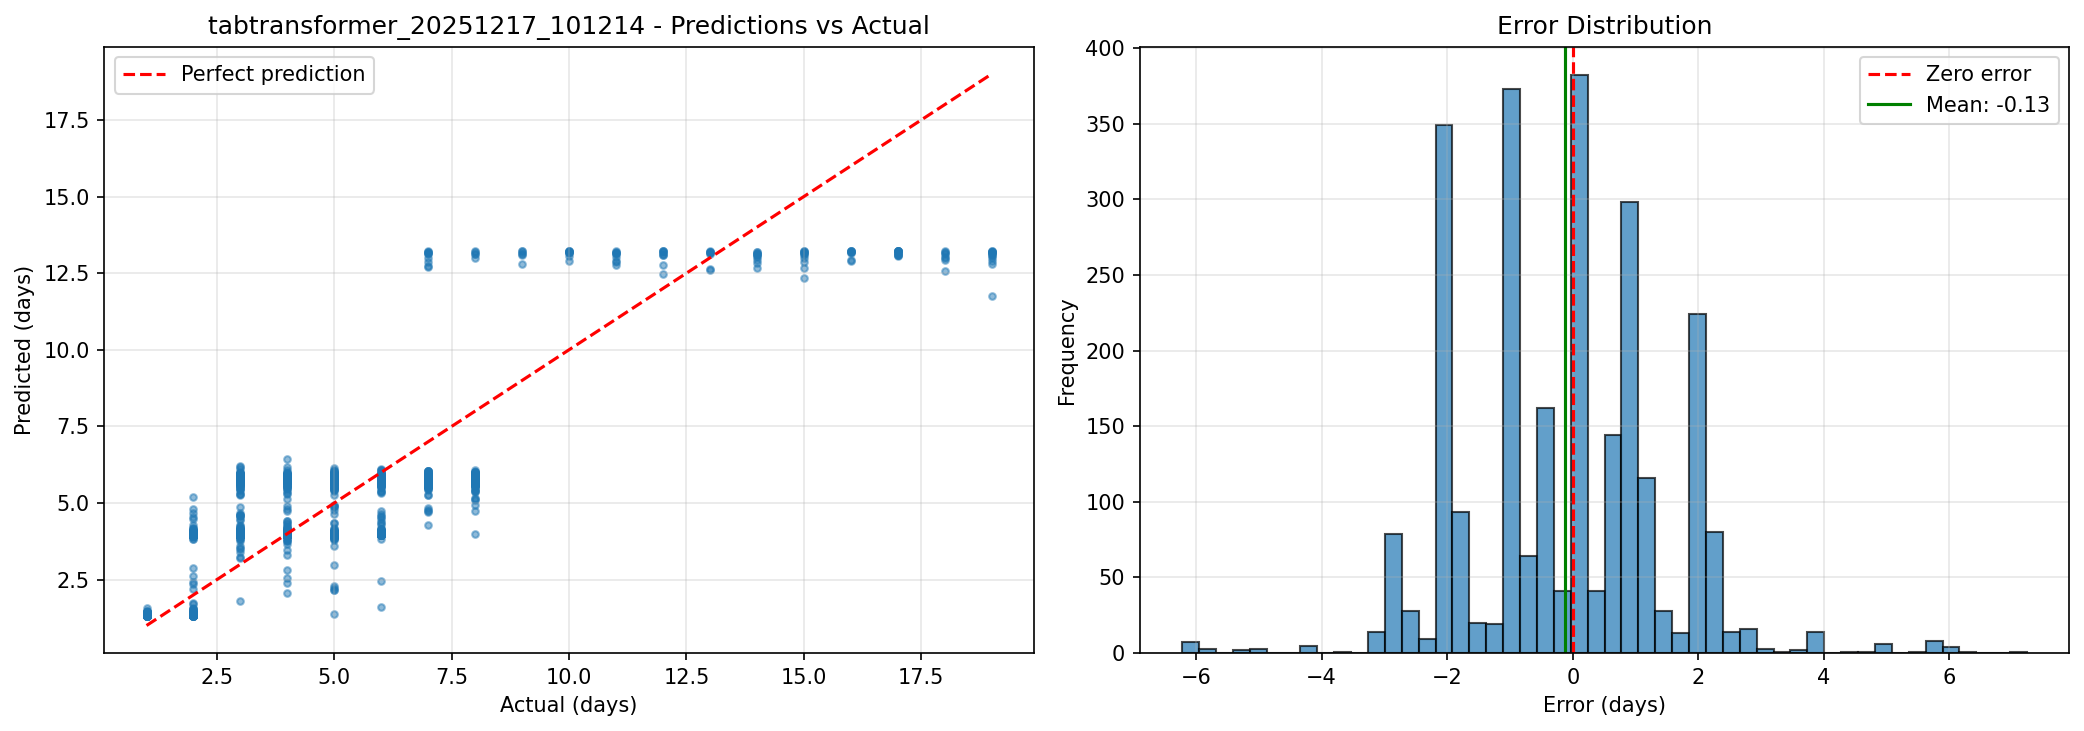
\includegraphics[width=\textwidth, height=0.82\textheight, keepaspectratio]{figures/tabtransformer_predictions.pdf}
    \end{center}
\end{frame}

%=============================================================================
\begin{frame}{TabTransformer -- Wykres Reszt}
    \begin{center}
        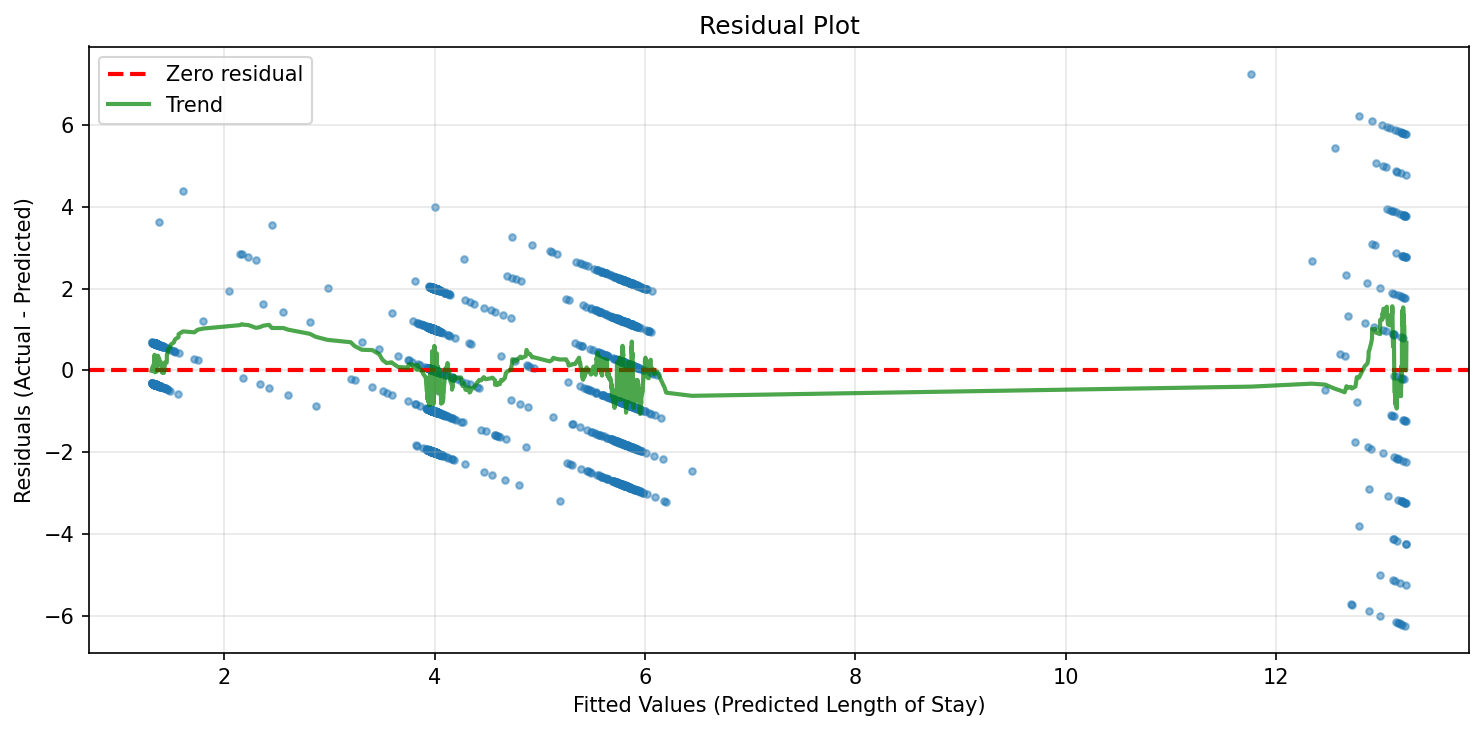
\includegraphics[width=\textwidth, height=0.82\textheight, keepaspectratio]{figures/tabtransformer_residuals.pdf}
    \end{center}
\end{frame}

%=============================================================================
\begin{frame}{Analiza najlepszego modelu -- TabNet}
    \begin{columns}[T]
        \begin{column}{0.5\textwidth}
            \textbf{Poprawa względem SimpleMLP:}
            \vspace{0.2cm}

            \small
            \begin{tabular}{lcc}
                \toprule
                Metryka   & Poprawa           \\
                \midrule
                MAE       & \textbf{-3.55\%}  \\
                RMSE      & \textbf{-4.64\%}  \\
                R²        & \textbf{+5.07\%}  \\
                Max Error & \textbf{-28.94\%} \\
                \bottomrule
            \end{tabular}

            \vspace{0.5cm}
            \textbf{Mocne strony:}
            \begin{itemize}
                \item Najniższy błąd (MAE = 1.26 dnia)
                \item Stabilność (std = 0.0006)
                \item Interpretowalność (attention)
            \end{itemize}
        \end{column}
        \begin{column}{0.5\textwidth}
            \textbf{Ograniczenia:}
            \begin{itemize}
                \item Trudności z pobytami >10 dni
                \item 33\% niewytłumaczonej wariancji
                \item Brak przedziałów ufności
            \end{itemize}

            \vspace{0.5cm}
            \textbf{Zastosowania:}
            \begin{itemize}
                \item Planowanie wykorzystania łóżek
                \item Zarządzanie personelem
                \item Analiza kosztów
            \end{itemize}
        \end{column}
    \end{columns}
\end{frame}

%=============================================================================
\begin{frame}{Wnioski}
    \begin{columns}[T]
        \begin{column}{0.5\textwidth}
            \textbf{Kluczowe obserwacje:}
            \begin{itemize}
                \item \textbf{TabNet} -- najlepszy model
                \item Specjalizowane architektury lepsze od MLP o 3-4\%
                \item Wszystkie modele: R² > 0.64
                \item Mechanizm attention kluczowy
            \end{itemize}

            \vspace{0.3cm}
            \textbf{Metodologia:}
            \begin{itemize}
                \item Grid Search + 5-fold CV
                \item 62 konfiguracje
                \item Reprodukowalne wyniki
            \end{itemize}
        \end{column}
        \begin{column}{0.5\textwidth}
            \textbf{Ranking architektur:}
            \vspace{0.2cm}

            \small
            \begin{tabular}{clc}
                \toprule
                \#                    & Architektura               & MAE                                \\
                \midrule
                \cellcolor{green!20}1 & \cellcolor{green!20}TabNet & \cellcolor{green!20}\textbf{1.264} \\
                2                     & TabTransformer             & 1.272                              \\
                3                     & SimpleMLP                  & 1.311                              \\
                \bottomrule
            \end{tabular}

            \vspace{0.5cm}
            \textbf{Możliwości poprawy:}
            \begin{itemize}
                \setlength{\itemsep}{0pt}
                \setlength{\parskip}{0pt}
                \item Rozszerzenie zbioru cech (historia choroby, leki)
                \item Oversampling długich pobytów (>10 dni)
                \item Przedziały ufności
            \end{itemize}
        \end{column}
    \end{columns}
\end{frame}

%=============================================================================
\begin{frame}{Dziękujemy za uwagę}
    \begin{center}
        \vspace{2cm}
        {\Huge\textbf{Dziękujemy za uwagę!}}

        \vspace{2cm}
        Kamil Selega (288780), Maria Słomiany (268576), Katarzyna Szczepaniak (261895)

        \vspace{0.3cm}
        Politechnika Wrocławska, Styczeń 2026
    \end{center}
\end{frame}

\end{document}
